\chapter{Resultados y discusión}

La composición de imágenes satelitales de radiancia en la Ciudad de México (Figura~\ref{radiancetrends}) muestra cualitativamente que los niveles más altos de radiancia se encuentran en la fracción norte-centro de la ciudad, lo que naturalmente, coincide con la mancha urbana. Dada esta distribución, se considera que un observador está <<dentro de la ciudad>> cuando se encuentra en alguno de los Sectores Urbanos mostrados en el Mapa CL-CDMX y <<fuera de la ciudad>> cuando está fuera de ellos, lo que corresponde con suelo de conservación. 

\section{Tendencias de radiancia en las alcaldías de la Ciudad de México}

Por efectos de representatividad se seleccionaron las siguientes figuras elaboradas con el software \textit{Radiance Light Trends} que muestran las tendencias de radiancia en la alcaldía Gustavo A. Madero (densamente poblada), Milpa Alta (menos poblada, con mayoría de territorio en suelo de conservación) y en el polígono de Ciudad Universitaria que contiene la REPSA. El resto de las tendencias por alcaldía se encuentran en el \textbf{\autoref{chap:anexos}}.

\begin{figure}[htb]
  \centering
    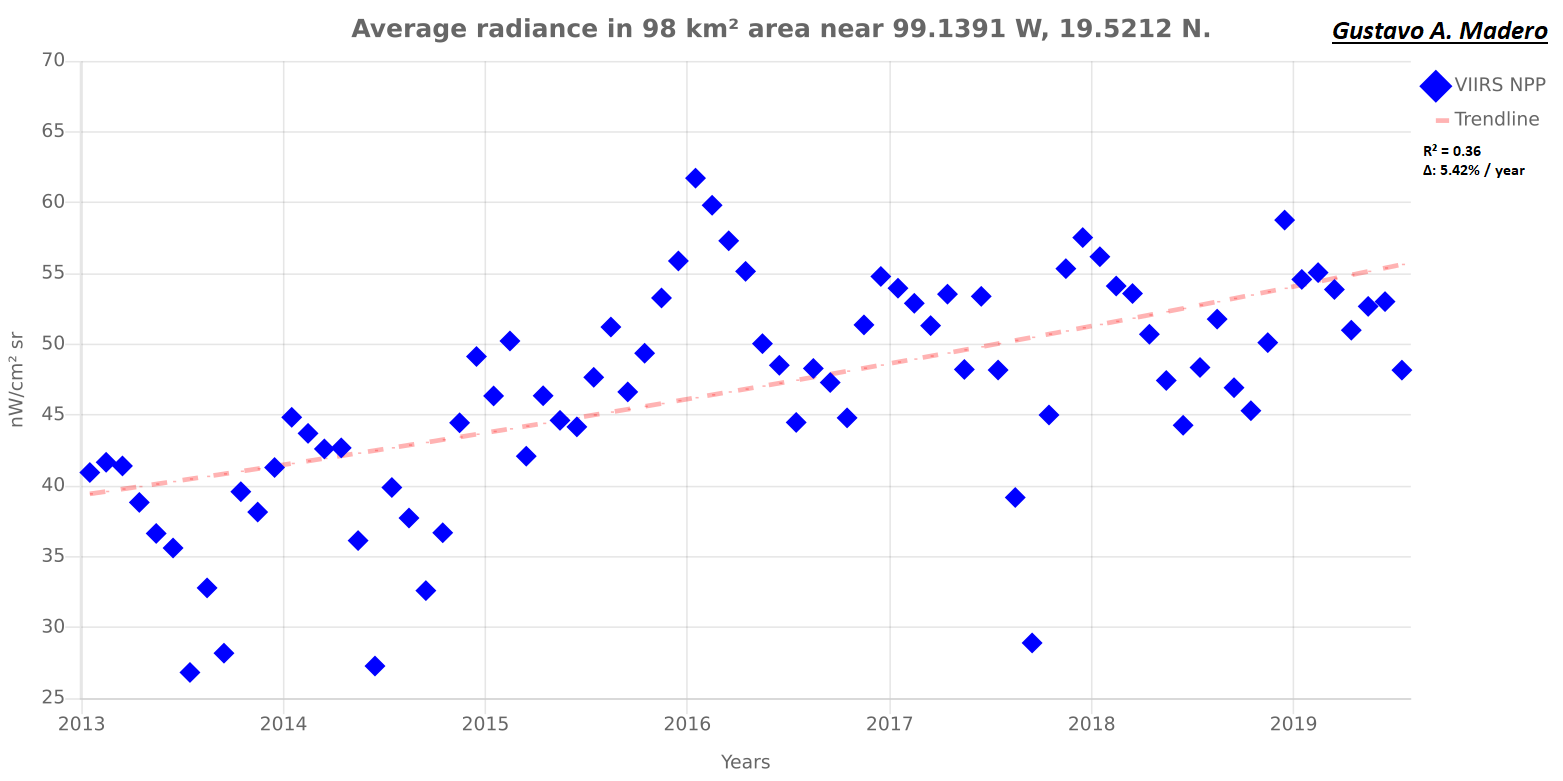
\includegraphics[width=1\textwidth]{GAM}
  \caption{Tendencia de radiancia promedio para la alcaldía Gustavo A. Madero}
  \label{radiancetrendsgam}
\end{figure}

\newpage


\begin{figure}[H]
  \centering
    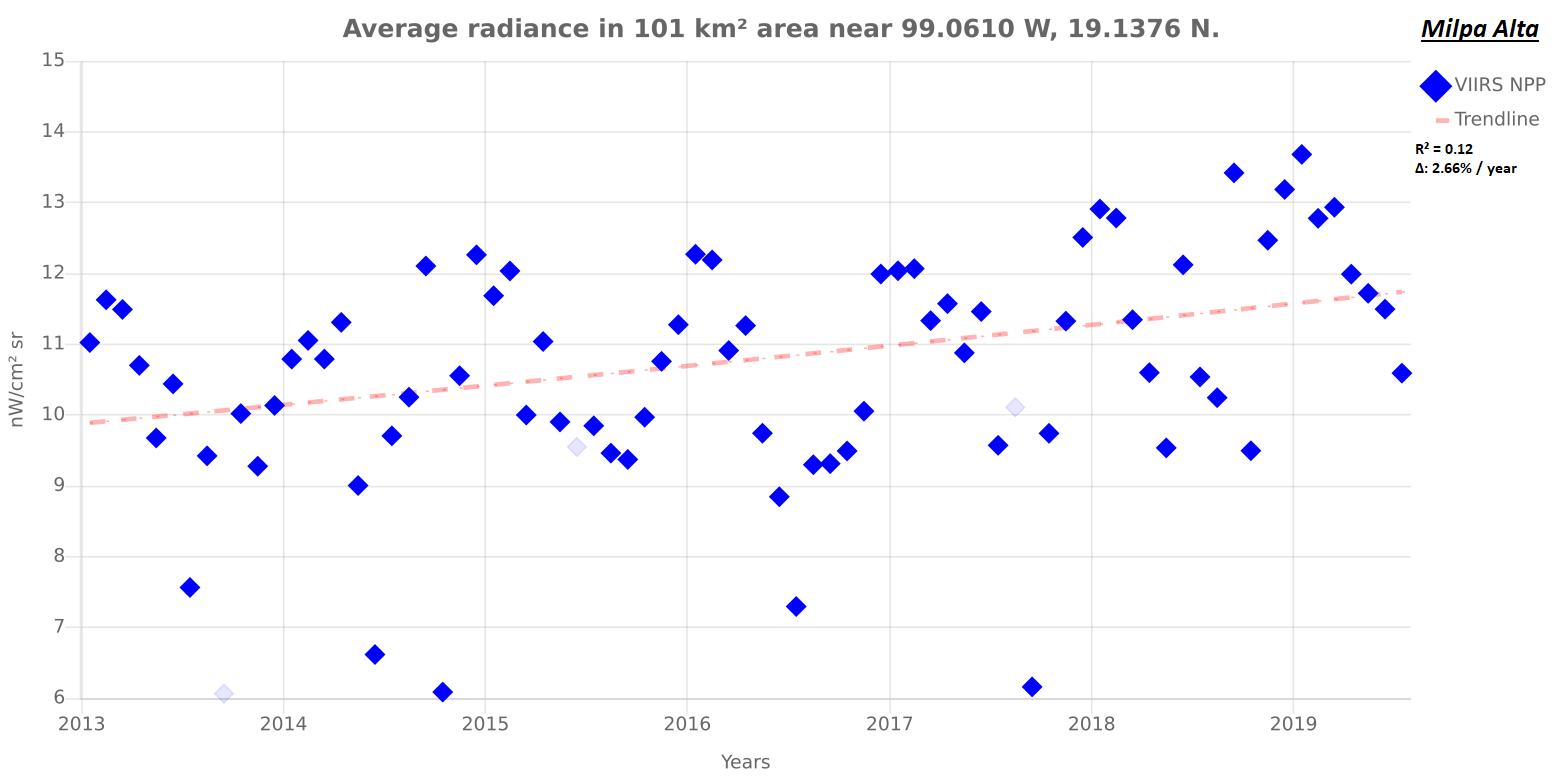
\includegraphics[width=1\textwidth]{MA}
  \caption{Tendencia de radiancia promedio para la alcaldía Milpa Alta}
  \label{radiancetrendsma}
\vspace{20mm} 
    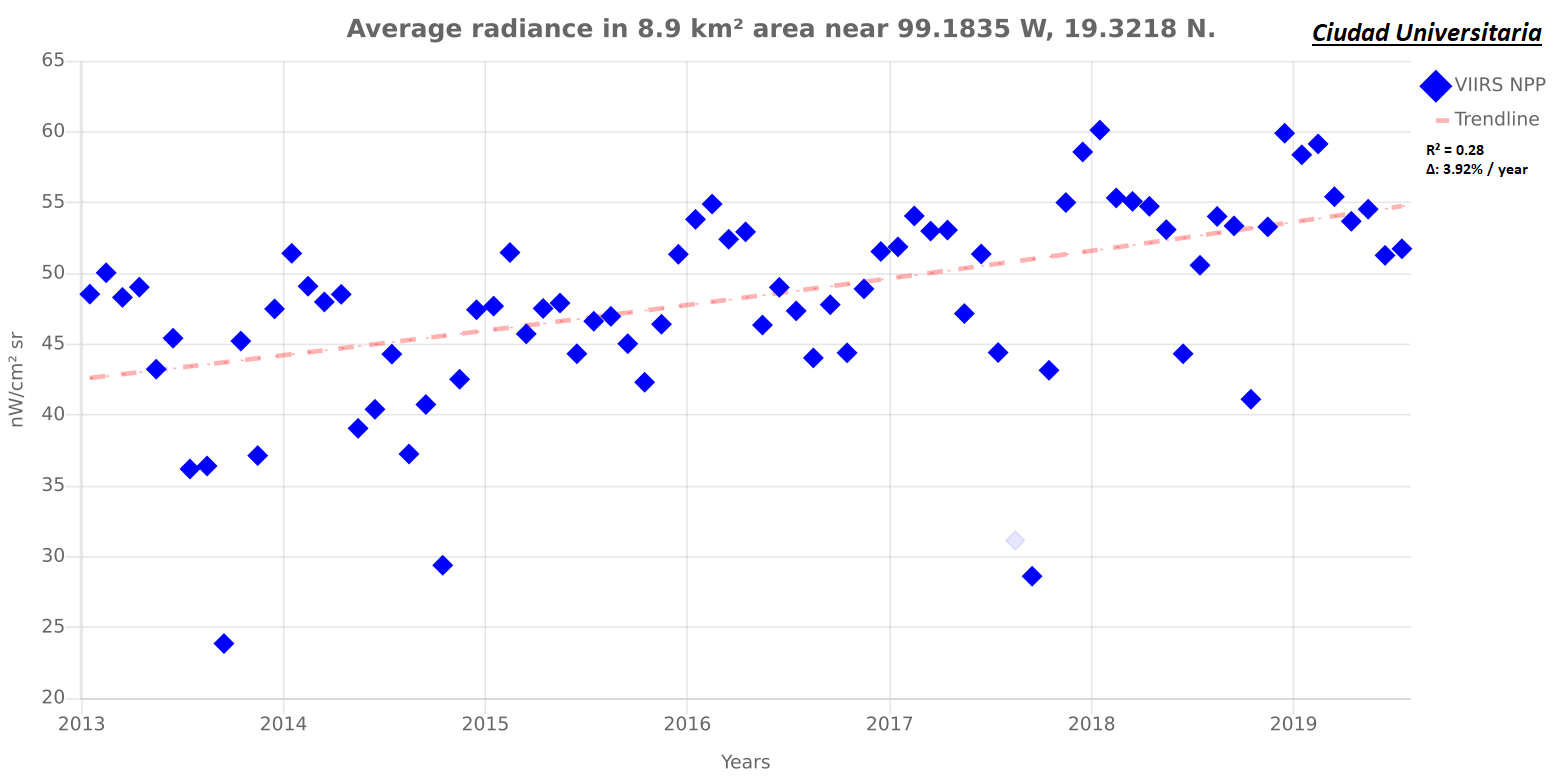
\includegraphics[width=1\textwidth]{CU}
  \caption{Tendencia de radiancia promedio para Ciudad Universitaria}
  \label{radiancetrendscu}
\end{figure}
\blindtext


\newpage

Como se muestra en el \textbf{Inventario de Alumbrado Público de la Ciudad de México}, el principal tipo de fuente de luz de la Ciudad de México es lámpara de halogenuros metálicos, sin embargo, siguiendo una tendencia mundial en las ciudades, podría aumentar exponencialmente el reemplazo por fuentes LED por el supuesto ahorro energético que esto implica.\\

Hablar sobre el cambio del programa de alumbrado.\\

No se puede comparar áreas tan grandes (caso de CU)

\newpage

\section{Mapa CL-CDMX}

\newpage

Espacio para explicar el mapa, hablar sobre la Sierra de Guadalupe, los sectores, polanco, etc.

\section{Gráficas tipo \textit{all sky} de distribución de radiancia}

blabla 

\newpage

lalalalalalala graficas
\newpage

\section{Experimentos numéricos}

blablabla

Por el potencial ahorro económico que supone, se está llevando a cabo una gran sustitución de instalaciones de alum-
brado público cambiando fuentes tradicionales -en muchos casos de vapor de sodio a alta presión- por LED.

\newpage

\subsection{Influencia del aerosol atmosférico en la distribución de radiancia}

\newpage

\subsection{Influencia de la nubosidad en la distribución de radiancia}

\newpage

\subsection{Cambio del tipo de luminarias en la Ciudad de México}

\newpage
